% Systematisk beskrivelse af konfigurations tabel.
En konfiguration af et system er en kombinering af elementer, og en konfigurations tabel beskriver den konfiguration.

Denne beskrivelse er baseret på Essence bogen afsnit 3.2, side 31 i PDF el. 16.
\winde{Lav en rigtig cite}

Systemets `use context' er at systemet bruges til at informere unipolare og bipolare patienter om der har været åbenbare adfærdsændringer. Udfordringen er så om mobilen kan bruges til at gøre dette ved hjælp af sensorer på mobilen.

Den øverste række i \cref{tab:konfigurationsTabel} navngiver de fire Views i Essence: Paradigm, Product, Project og Process.

`Focus' rækken repræsenterer de største problemer og løsninger i projektet. 
Udfordringen er tiltænkt til at være om man kan bruge en mobil til at overvåge adfærd af unipolare og bipolare patienter og gøre dem opmærksom på adfærdsændringer og dette er så tiltænkt at disse patienter åbner en applikation på denne mobil hvor de vil blive blive givet et overblik og derved få at vide om der har været adfærdsændringer. 
Det er så vigtigt at systemet skal kun observere og informere og derved bruge konceptet 'patient empowerment'.
Løsnings strategien er så at bruge en smartphone, og udvikle et system som kan registrere data fra forskellige sensor moduler og gemme det på telefonen som den bliver brugt af patienten.
Data den indsamler skal være objektiv, så idéen er at den skal fungere som en objektiv dagbog.
Denne data kan så bruges til analyse og blive undersøgt om der er nogle ændringer i patientens opførsel og skal let kunne aflæses af patienten hvorfra de kan få relevant information fra den præsenterede data. 

`Overview' rækken repræsenterer projektets stakeholders. Hoved perspektivet er selvfølgelig fra patienterne, da det er dem som skal bruge produktet men der er også sponsorer som er interesseret i at se projektet være en succes da det vil gøre at deres patienter vil få det nemmere. 
Designet på projektet er simpelt idet at der bruges mobil eller wearables til sensor input og at denne data så gemmes og analyseres på mobilen. 
For at evaluere denne funktionalitet kan der bruges fokusgrupper og usability tests til at finde ud af om den er akkurat, let-tilgængelig og forståelig.

`Details' rækken repræsenterer nøgle scenarier, nøgle componenter og features.
Der blev fundet ud af at der kan være huller i data ... \lasse{Skriv noget om findings her?}

\begin{figure}[h]
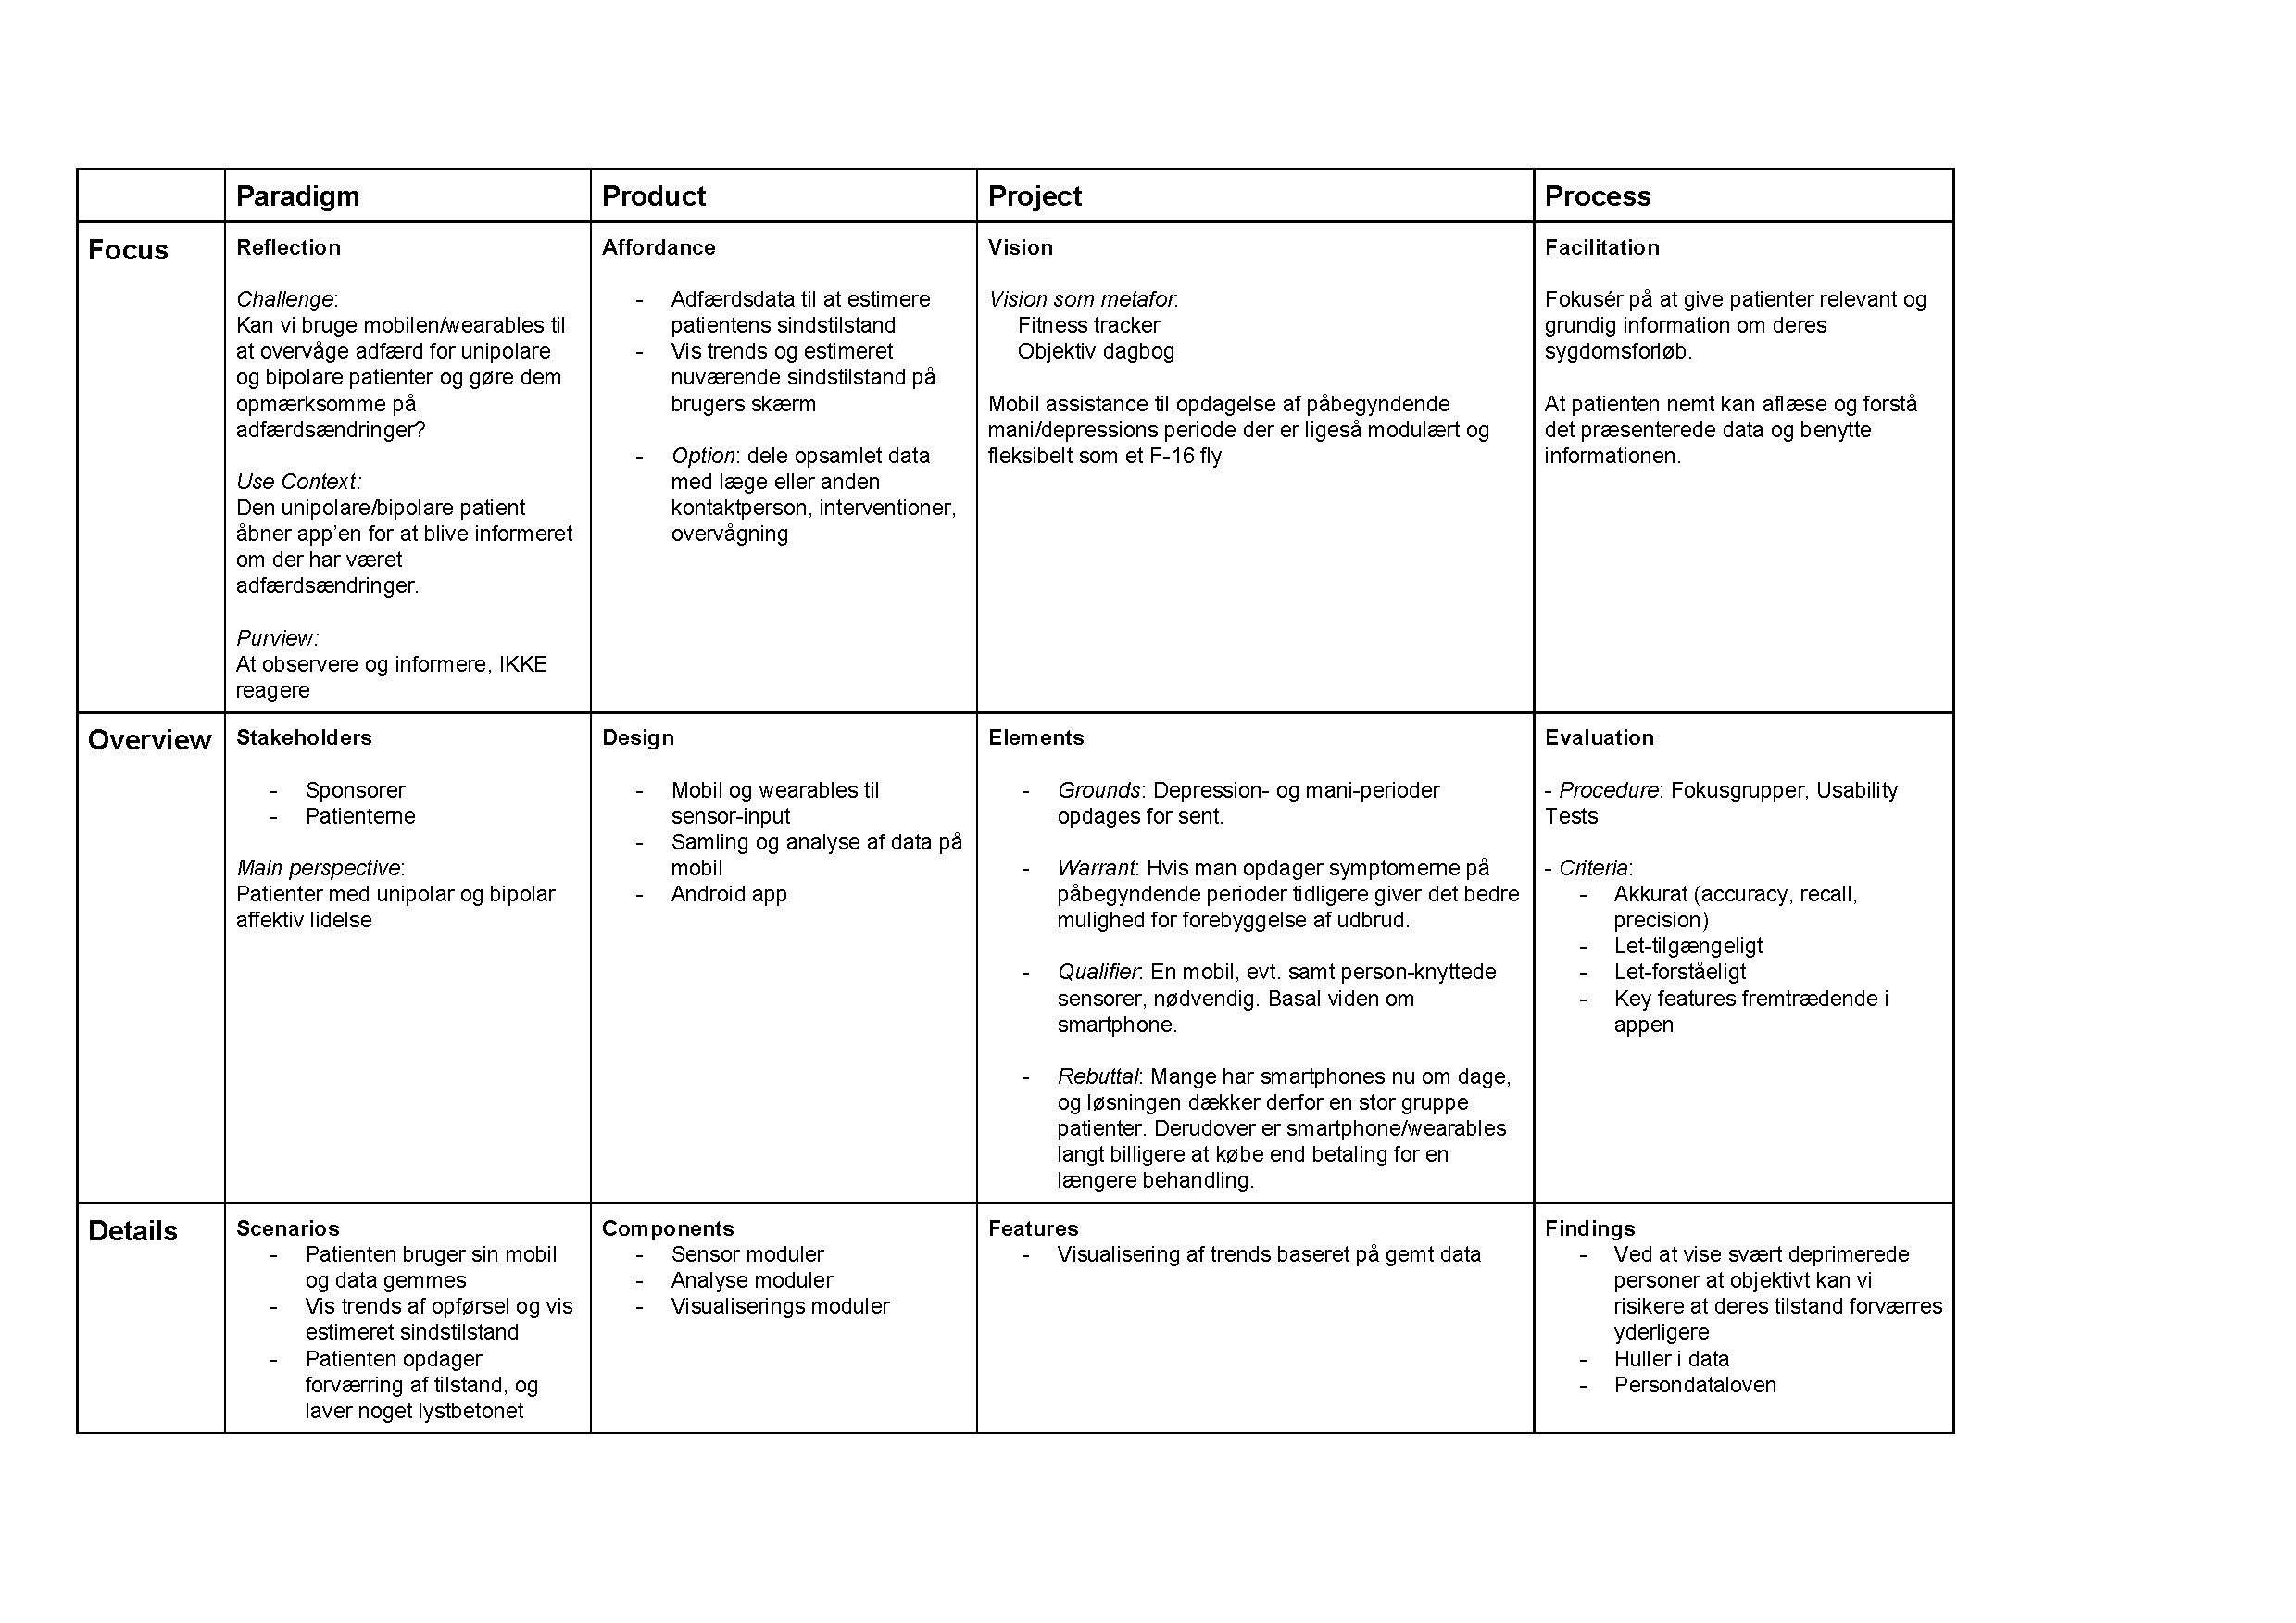
\includegraphics[scale = 0.45,trim = 1cm 3cm 6cm 2cm, clip]{KonfigurationTabel}
\caption{Konfigurations tabellen for systemet.}
\label{tab:konfigurationsTabel}
\end{figure}
